\documentclass{article}

\title{Homework \#4}
\author{Illya Starikov}
\date{Due Date: March 23, 2016}

\usepackage{booktabs}
\usepackage[table]{xcolor}
\usepackage{listings}

\usepackage{tikz}
\usepackage{tkz-graph}
\usetikzlibrary{arrows}
\usetikzlibrary{calc}

\newcommand{\ak}{\cellcolor{gray!50}}
\newcommand{\aky}{\cellcolor{red!50}}
\newcommand{\akn}{\cellcolor{gray!15}}

\newcolumntype{P}[1]{>{\centering\arraybackslash}p{#1}}

\begin{document}
\maketitle

\section{Activity Selection Problem}
Plotting this out on a graph,

\begin{center}
\begin{tabular}{l|P{.20cm}|P{.20cm}|P{.20cm}|P{.20cm}|P{.20cm}|P{.20cm}|P{.20cm}|P{.20cm}|P{.20cm}|P{.20cm}|P{.20cm}|P{.20cm}|P{.20cm}|P{.20cm}|P{.20cm}}
    \toprule
    & 0 & 1 & 2 & 3 & 4 & 5 & 6 & 7 & 8 & 9 & 10 & 11 & 12 & 13 & 14 \\ \hline
    $a_1$ & & \ak & \ak & \ak & \ak & & & & & & & & & & \\
    $a_2$ & & & & \ak & \ak & \ak & & & & & & & & & \\
    $a_3$ & \ak & \ak & \ak & \ak & \ak & \ak & \ak & & & & & & & & \\
    $a_4$ & & & & & & \ak & \ak & \ak & & & & & & & \\
    $a_5$ & & & & \ak & \ak & \ak & \ak & \ak & \ak & & & & & & \\
    $a_6$ & & & & & & \ak & \ak & \ak & \ak & \ak & & & & & \\
    $a_7$ & & & & & & & \ak & \ak & \ak & \ak & \ak & & & & \\
    $a_8$ & & & & & & & & & \ak & \ak & \ak & \ak & & & \\
    $a_9$ & & & & & & & & & \ak & \ak & \ak & \ak & \ak & & \\
    $a_{10}$ & & & \ak & \ak & \ak & \ak & \ak & \ak & \ak & \ak & \ak & \ak & \ak & \ak & \\
    $a_{11}$ & & & & & & & & & & & & & \ak & \ak & \ak \\
    \bottomrule
\end{tabular}
\end{center}

We can plainly see the optimal solution to be $\{ a_1, a_4, a_8, a_{11} \}$. We get this solution by using the ending first greedy algorithm. Here are the steps to obtain the solution.

\begin{center}
\begin{tabular}{l|P{.20cm}|P{.20cm}|P{.20cm}|P{.20cm}|P{.20cm}|P{.20cm}|P{.20cm}|P{.20cm}|P{.20cm}|P{.20cm}|P{.20cm}|P{.20cm}|P{.20cm}|P{.20cm}|P{.20cm}}
    \toprule
    & 0 & 1 & 2 & 3 & 4 & 5 & 6 & 7 & 8 & 9 & 10 & 11 & 12 & 13 & 14 \\ \hline
    $a_1$ & & \aky & \aky & \aky & \aky & & & & & & & & & & \\
    $a_2$ & & & & \ak & \ak & \ak & & & & & & & & & \\
    $a_3$ & \ak & \ak & \ak & \ak & \ak & \ak & \ak & & & & & & & & \\
    $a_4$ & & & & & & \ak & \ak & \ak & & & & & & & \\
    $a_5$ & & & & \ak & \ak & \ak & \ak & \ak & \ak & & & & & & \\
    $a_6$ & & & & & & \ak & \ak & \ak & \ak & \ak & & & & & \\
    $a_7$ & & & & & & & \ak & \ak & \ak & \ak & \ak & & & & \\
    $a_8$ & & & & & & & & & \ak & \ak & \ak & \ak & & & \\
    $a_9$ & & & & & & & & & \ak & \ak & \ak & \ak & \ak & & \\
    $a_{10}$ & & & \ak & \ak & \ak & \ak & \ak & \ak & \ak & \ak & \ak & \ak & \ak & \ak & \\
    $a_{11}$ & & & & & & & & & & & & & \ak & \ak & \ak \\
    \bottomrule
\end{tabular}
\end{center}

\begin{center}
\begin{tabular}{l|P{.20cm}|P{.20cm}|P{.20cm}|P{.20cm}|P{.20cm}|P{.20cm}|P{.20cm}|P{.20cm}|P{.20cm}|P{.20cm}|P{.20cm}|P{.20cm}|P{.20cm}|P{.20cm}|P{.20cm}}
    \toprule
    & 0 & 1 & 2 & 3 & 4 & 5 & 6 & 7 & 8 & 9 & 10 & 11 & 12 & 13 & 14 \\ \hline
    $a_1$ & & \aky & \aky & \aky & \aky & & & & & & & & & & \\
    $a_2$ & & & & \akn & \akn & \akn & & & & & & & & & \\
    $a_3$ & \akn & \akn & \akn & \akn & \akn & \akn & \akn & & & & & & & & \\
    $a_4$ & & & & & & \aky & \aky & \aky & & & & & & & \\
    $a_5$ & & & & \ak & \ak & \ak & \ak & \ak & \ak & & & & & & \\
    $a_6$ & & & & & & \ak & \ak & \ak & \ak & \ak & & & & & \\
    $a_7$ & & & & & & & \ak & \ak & \ak & \ak & \ak & & & & \\
    $a_8$ & & & & & & & & & \ak & \ak & \ak & \ak & & & \\
    $a_9$ & & & & & & & & & \ak & \ak & \ak & \ak & \ak & & \\
    $a_{10}$ & & & \ak & \ak & \ak & \ak & \ak & \ak & \ak & \ak & \ak & \ak & \ak & \ak & \\
    $a_{11}$ & & & & & & & & & & & & & \ak & \ak & \ak \\
    \bottomrule
\end{tabular}
\end{center}

\begin{center}
\begin{tabular}{l|P{.20cm}|P{.20cm}|P{.20cm}|P{.20cm}|P{.20cm}|P{.20cm}|P{.20cm}|P{.20cm}|P{.20cm}|P{.20cm}|P{.20cm}|P{.20cm}|P{.20cm}|P{.20cm}|P{.20cm}}
    \toprule
    & 0 & 1 & 2 & 3 & 4 & 5 & 6 & 7 & 8 & 9 & 10 & 11 & 12 & 13 & 14 \\ \hline
    $a_1$ & & \aky & \aky & \aky & \aky & & & & & & & & & & \\
    $a_2$ & & & & \akn & \akn & \akn & & & & & & & & & \\
    $a_3$ & \akn & \akn & \akn & \akn & \akn & \akn & \akn & & & & & & & & \\
    $a_4$ & & & & & & \aky & \aky & \aky & & & & & & & \\
    $a_5$ & & & & \akn & \akn & \akn & \akn & \akn & \akn & & & & & & \\
    $a_6$ & & & & & & \akn & \akn & \akn & \akn & \akn & & & & & \\
    $a_7$ & & & & & & & \akn & \akn & \akn & \akn & \akn & & & & \\
    $a_8$ & & & & & & & & & \aky & \aky & \aky & \aky & & & \\
    $a_9$ & & & & & & & & & \ak & \ak & \ak & \ak & \ak & & \\
    $a_{10}$ & & & \ak & \ak & \ak & \ak & \ak & \ak & \ak & \ak & \ak & \ak & \ak & \ak & \\
    $a_{11}$ & & & & & & & & & & & & & \ak & \ak & \ak \\
    \bottomrule
\end{tabular}
\end{center}

\begin{center}
\begin{tabular}{l|P{.20cm}|P{.20cm}|P{.20cm}|P{.20cm}|P{.20cm}|P{.20cm}|P{.20cm}|P{.20cm}|P{.20cm}|P{.20cm}|P{.20cm}|P{.20cm}|P{.20cm}|P{.20cm}|P{.20cm}}
    \toprule
    & 0 & 1 & 2 & 3 & 4 & 5 & 6 & 7 & 8 & 9 & 10 & 11 & 12 & 13 & 14 \\ \hline
    $a_1$ & & \aky & \aky & \aky & \aky & & & & & & & & & & \\
    $a_2$ & & & & \akn & \akn & \akn & & & & & & & & & \\
    $a_3$ & \akn & \akn & \akn & \akn & \akn & \akn & \akn & & & & & & & & \\
    $a_4$ & & & & & & \aky & \aky & \aky & & & & & & & \\
    $a_5$ & & & & \akn & \akn & \akn & \akn & \akn & \akn & & & & & & \\
    $a_6$ & & & & & & \akn & \akn & \akn & \akn & \akn & & & & & \\
    $a_7$ & & & & & & & \akn & \akn & \akn & \akn & \akn & & & & \\
    $a_8$ & & & & & & & & & \aky & \aky & \aky & \aky & & & \\
    $a_9$ & & & & & & & & & \akn & \akn & \akn & \akn & \akn & & \\
    $a_{10}$ & & & \akn & \akn & \akn & \akn & \akn & \akn & \akn & \akn & \akn & \akn & \akn & \akn & \\
    $a_{11}$ & & & & & & & & & & & & & \aky & \aky & \aky \\
    \bottomrule
\end{tabular}
\end{center}

\section{Graph And Depth First Search}
\begin{center}
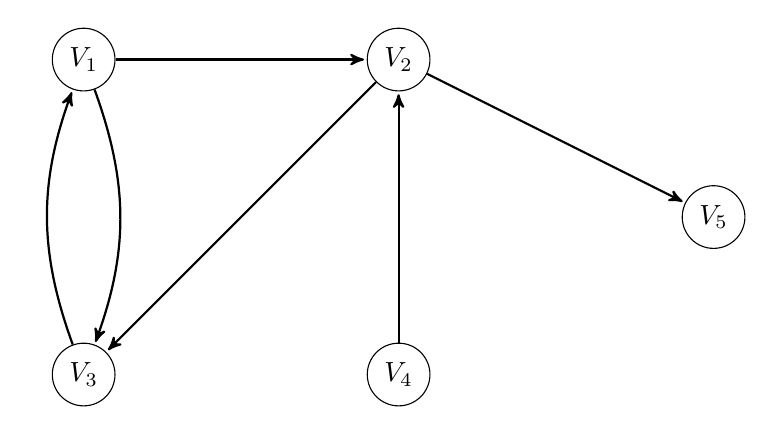
\begin{tikzpicture}[>=stealth',shorten >=1pt,auto,node distance=2.8cm]
    \node[shape=circle,draw=black] (1) at (0,0) {$V_1$};
    \node[shape=circle,draw=black] (2) at (4,0) {$V_2$};
    \node[shape=circle,draw=black] (3) at (0,-4) {$V_3$};
    \node[shape=circle,draw=black] (4) at (4,-4) {$V_4$};
    \node[shape=circle,draw=black] (5) at (8,-2) {$V_5$};

    \path [->,thick] (1) edge node[left] {} (2);
    \path [->,thick] (1) edge [bend left=20] node[left] {} (3);

    \path [->,thick] (2) edge node[left] {} (5);
    \path [->,thick] (2) edge node[left] {} (3);

    \path [->,thick] (3) edge [bend left=20] node[left] {} (1);

    \path [->,thick] (4) edge node[left] {} (2);
\end{tikzpicture}
\end{center}

\subsection{Depth First Search}
\begin{center}
\begin{tabular}{rccccc}
    \textbf{Ouput}:    & $V_1$ & $V_2$ & $V_3$ & $V_5$ & $V_4$\\
    \textbf{Distance}: & 0 & 1 & 1 & 2 & $\infty$
\end{tabular}
\end{center}

\subsubsection{Queue Status}
\begin{tabular}{|ll}
    \hline
    $V_1$ & \\
    \hline
\end{tabular}

\noindent
\begin{tabular}{|lll}
    \hline
    $V_2$ & $V_3$ \\
    \hline
\end{tabular}

\noindent
\begin{tabular}{|lll}
    \hline
    $V_3$ & $V_5$ \\
    \hline
\end{tabular}

\noindent
\begin{tabular}{|ll}
    \hline
    $V_5$ & \\
    \hline
\end{tabular}

\noindent
\begin{tabular}{|ll}
    \hline
     & \\
    \hline
\end{tabular}

\noindent
\begin{tabular}{|ll}
    \hline
     $V_4$ & \\
    \hline
\end{tabular}

\noindent
\begin{tabular}{|ll}
    \hline
     & \\
    \hline
\end{tabular}
\section{Depth First Search and Topological Sorting}
\begin{center}
\begin{tabular}{c|cc}
    \toprule
    \textbf{Ouput} & \textbf{Discovery} & \textbf{Finish} \\ \hline
    a & 1 & 10 \\
    c & 2 & 9\\
    d & 3 & 4\\
    e & 5 & 8\\
    h & 6 & 7\\
    b & 11 & 12\\
    f & 13 & 16\\
    g & 14 & 15\\
    \bottomrule
\end{tabular}
\end{center}

\subsubsection{Queue Status}
\begin{center}
\begin{tabular}{|l|}
    \\ a \\
    \hline
\end{tabular} $\rightarrow$
\begin{tabular}{|l|}
    \\ d \\ c \\ a \\
    \hline
\end{tabular} $\rightarrow$
\begin{tabular}{|l|}
    \\ c \\ a \\
    \hline
\end{tabular} $\rightarrow$
\begin{tabular}{|l|}
    \\ e \\ c \\ a \\
    \hline
\end{tabular} $\rightarrow$
\begin{tabular}{|l|}
    \\ h \\ e \\ c \\ a \\
    \hline
\end{tabular} $\rightarrow$
\begin{tabular}{|l|}
    \\ e \\ c \\ a \\
    \hline
\end{tabular} $\rightarrow$
\begin{tabular}{|l|}
    \\ c \\ a \\
    \hline
\end{tabular} $\rightarrow$
\begin{tabular}{|l|}
    \\ a \\
    \hline
\end{tabular} $\rightarrow$
\begin{tabular}{|l|}
     \\
    \hline
\end{tabular} $\rightarrow$
\begin{tabular}{|l|}
    \\ b \\
    \hline
\end{tabular}

\noindent
$\rightarrow$
\begin{tabular}{|l|}
    \\
    \hline
\end{tabular} $\rightarrow$
\begin{tabular}{|l|}
    \\ f \\
    \hline
\end{tabular} $\rightarrow$
\begin{tabular}{|l|}
    \\ g \\ f \\
    \hline
\end{tabular} $\rightarrow$
\begin{tabular}{|l|}
    \\ f \\
    \hline
\end{tabular} $\rightarrow$
\begin{tabular}{|l|}
    \\
    \hline
\end{tabular}
\end{center}

\subsubsection{Edge Classification}
\begin{center}
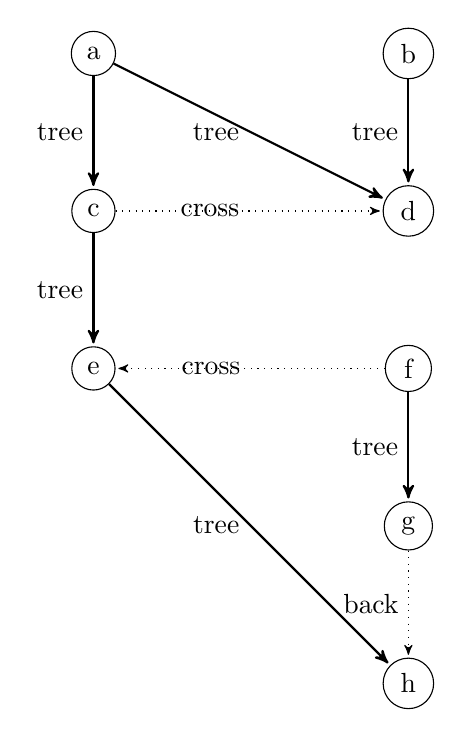
\begin{tikzpicture}[>=stealth',shorten >=1pt,auto,node distance=2.8cm]
    \node[shape=circle,draw=black] (a) at (0,0) {a};
    \node[shape=circle,draw=black] (b) at (4,0) {b};

    \node[shape=circle,draw=black] (c) at (0,-2) {c};
    \node[shape=circle,draw=black] (d) at (4,-2) {d};

    \node[shape=circle,draw=black] (e) at (0,-4) {e};
    \node[shape=circle,draw=black] (f) at (4,-4) {f};

    \node[shape=circle,draw=black] (g) at (4,-6) {g};
    \node[shape=circle,draw=black] (h) at (4,-8) {h};

    \path [->,thick] (a) edge node[left] {tree} (d);
    \path [->,thick] (a) edge node[left] {tree} (c);

    \path [->,thick] (b) edge node[left] {tree} (d);

    \path [->,dotted] (c) edge node[left] {cross} (d);
    \path [->,thick] (c) edge node[left] {tree} (e);

    \path [->,thick] (e) edge node[left] {tree} (h);

    \path [->,dotted] (f) edge node[left] {cross} (e);
    \path [->,thick] (f) edge node[left] {tree} (g);

    \path [->,dotted] (g) edge node[left] {back} (h);
\end{tikzpicture}
\end{center}

\subsubsection{Topological Sorting}
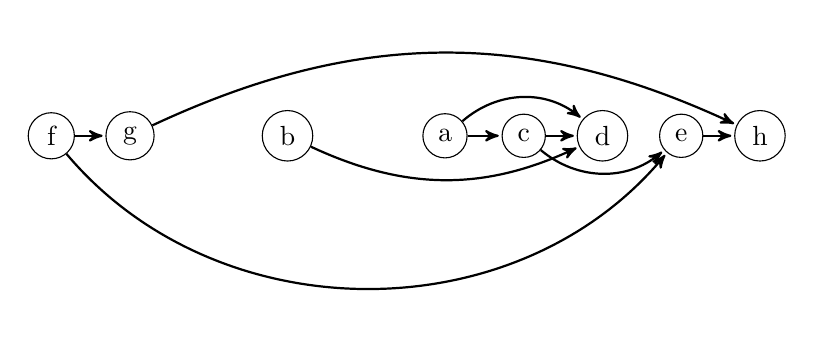
\begin{tikzpicture}[>=stealth',shorten >=1pt,auto,node distance=2.8cm]
    \node[shape=circle,draw=black] (f) at (0,0) {f};
    \node[shape=circle,draw=black] (g) at (1,0) {g};

    \node[shape=circle,draw=black] (b) at (3,0) {b};

    \node[shape=circle,draw=black] (a) at (5,0) {a};
    \node[shape=circle,draw=black] (c) at (6,0) {c};
    \node[shape=circle,draw=black] (d) at (7,0) {d};
    \node[shape=circle,draw=black] (e) at (8,0) {e};
    \node[shape=circle,draw=black] (h) at (9,0) {h};

    \path [->,thick] (f) edge node[left] {} (g);
    \path [->,thick] (g) edge[bend left=25] node[left] {} (h);
    \path [->,thick] (f) edge[bend right = 50] node[left] {} (e);

    \path [->,thick] (b) edge[bend right=25] node[left] {} (d);

    \path [->,thick] (a) edge node[left] {} (c);
    \path [->,thick] (a) edge[bend left=40] node[left] {} (d);
    \path [->,thick] (c) edge node[left] {} (d);
    \path [->,thick] (c) edge[bend right=40] node[left] {} (e);
    \path [->,thick] (e) edge node[left] {} (h);
\end{tikzpicture}


\section{Kruskal's and Prim's Algorithm}
Please note that my tables are different, however the algorithm is the same is the same.

\subsection{Kruskal}
Kruskal's works the same way, except my column headers are more verbose and there an Iteration Number column, making it easy to keep track of large algorithms.

\begin{center}
\begin{tabular}{c|c|c|c}
    \toprule
    \textbf{Iteration Number} & \textbf{Edge} & \textbf{Weight} & \textbf{Action Taken} \\ \hline
    1 & $\{u, \ y\}$ & 1 & Added \\
    1 & $\{u, \ x\}$ & 1 & Added \\
    2 & $\{s, \ t\}$ & 2 & Added  \\
    3 & $\{t, \ y\}$ & 2 & Added  \\
    4 & $\{s, \ u\}$ & 3 & Not Added  \\
    5 & $\{s, \ x\}$ & 3 & Not Added  \\
    6 & $\{t, \ x\}$ & 3 & Not Added  \\
    \bottomrule
\end{tabular}
\end{center}

\subsection{Prim}
Prim's is also the same, with the exception that my headers are also verbose and the table is sorted linearly by the vertexes and edges that are added. The process is still the same of starting a vertex and branching out based on the best possible choice at the moment.

\begin{center}
\begin{tabular}{c|c|c|c}
    \toprule
    \textbf{Iteration Number} & \textbf{Vertex Added} & \textbf{Edge Added} & \textbf{Weight} \\ \hline
    0 & $s$ &              &   \\
    1 & $t$ & $\{s, \ t\}$ & 2 \\
    2 & $x$ & $\{t, \ y\}$ & 2 \\
    3 & $u$ & $\{y, \ u\}$ & 1 \\
    4 & $y$ & $\{u, \ x\}$ & 1 \\
    \bottomrule
\end{tabular}
\end{center}

Both algorithms produce the same result.

\end{document}